\documentclass[12pt,a4paper]{book}

% ═══════════════════════════════════════════
% PACKAGES
% ═══════════════════════════════════════════
\usepackage[utf8]{inputenc}
\usepackage[T1]{fontenc}
\usepackage{lmodern}
\usepackage{amsmath,amssymb,amsthm,amsfonts}
\usepackage{mathtools}
\usepackage{tikz}
\usetikzlibrary{arrows.meta,positioning,calc,decorations.pathmorphing}
\usepackage{pgfplots}
\pgfplotsset{compat=1.18}
\usepackage{tcolorbox}
\tcbuselibrary{theorems,skins,breakable}
\usepackage{enumitem}
\usepackage{fancyhdr}
\usepackage{titlesec}
\usepackage{geometry}
\usepackage{hyperref}
\usepackage{xcolor}
\usepackage{booktabs}
\usepackage{multicol}
\usepackage{etoolbox}

% ═══════════════════════════════════════════
% PAGE LAYOUT
% ═══════════════════════════════════════════
\geometry{a4paper,margin=2.5cm,top=3cm,bottom=3cm}

% ═══════════════════════════════════════════
% COLORS
% ═══════════════════════════════════════════
\definecolor{deepblue}{HTML}{1a1a6e}
\definecolor{accentblue}{HTML}{4a47a3}
\definecolor{lightblue}{HTML}{e8e8f8}
\definecolor{prereqbg}{HTML}{fff8e1}
\definecolor{prereqborder}{HTML}{f9a825}
\definecolor{examplebg}{HTML}{e8f5e9}
\definecolor{exampleborder}{HTML}{43a047}
\definecolor{warningbg}{HTML}{fce4ec}
\definecolor{warningborder}{HTML}{e53935}
\definecolor{thmblue}{HTML}{1565c0}
\definecolor{defgreen}{HTML}{2e7d32}

% ═══════════════════════════════════════════
% HEADERS & FOOTERS
% ═══════════════════════════════════════════
\pagestyle{fancy}
\fancyhf{}
\fancyhead[LE]{\textit{\nouppercase{\leftmark}}}
\fancyhead[RO]{\textit{\nouppercase{\rightmark}}}
\fancyfoot[C]{\thepage}
\renewcommand{\headrulewidth}{0.4pt}

% ═══════════════════════════════════════════
% CHAPTER & SECTION STYLING
% ═══════════════════════════════════════════
\titleformat{\chapter}[display]
  {\normalfont\Huge\bfseries\color{deepblue}}
  {\chaptertitlename\ \thechapter}{20pt}{\Huge}
\titleformat{\section}
  {\normalfont\Large\bfseries\color{accentblue}}
  {\thesection}{1em}{}
\titleformat{\subsection}
  {\normalfont\large\bfseries\color{accentblue!80!black}}
  {\thesubsection}{1em}{}

% ═══════════════════════════════════════════
% THEOREM ENVIRONMENTS
% ═══════════════════════════════════════════
\newtcbtheorem[number within=section]{theorem}{Theorem}{
  colback=lightblue,colframe=thmblue,
  fonttitle=\bfseries,
  breakable,
  before upper={\parindent15pt},
}{thm}

\newtcbtheorem[number within=section]{definition}{Definition}{
  colback=lightblue!30,colframe=defgreen,
  fonttitle=\bfseries,
  breakable,
  before upper={\parindent15pt},
}{def}

\newtcbtheorem[number within=section]{lemma}{Lemma}{
  colback=lightblue!20,colframe=accentblue!70,
  fonttitle=\bfseries,
  breakable,
}{lem}

% Prerequisite box
\newtcolorbox{prereqbox}{
  colback=prereqbg,colframe=prereqborder,
  title={\textbf{Prerequisites — What You Need to Know}},
  fonttitle=\bfseries\color{black},
  breakable,
  left=8pt,right=8pt,
  boxrule=1.5pt,
  arc=4pt,
}

% Example box
\newtcolorbox{examplebox}[1][]{
  colback=examplebg!30,colframe=exampleborder,
  title={\textbf{Worked Example} #1},
  fonttitle=\bfseries\color{black},
  breakable,
  left=8pt,right=8pt,
  boxrule=1pt,
  arc=4pt,
}

% Important note box
\newtcolorbox{importantbox}{
  colback=warningbg!30,colframe=warningborder,
  title={\textbf{Important — Exam Alert!}},
  fonttitle=\bfseries\color{black},
  breakable,
  boxrule=1pt,arc=4pt,
}

% Proof environment
\renewcommand{\qedsymbol}{$\blacksquare$}

% ═══════════════════════════════════════════
% DOCUMENT
% ═══════════════════════════════════════════
\begin{document}

% ─── COVER PAGE ───
\begin{titlepage}
\begin{tikzpicture}[remember picture,overlay]
  \fill[deepblue] (current page.south west) rectangle (current page.north east);
  \node[anchor=center,white,font=\fontsize{48}{56}\selectfont\bfseries] 
    at ([yshift=4cm]current page.center) {MSc Mathematics};
  \node[anchor=center,white,font=\fontsize{28}{34}\selectfont] 
    at ([yshift=1.5cm]current page.center) {Semester 1 --- Complete Study Guide};
  \draw[white,line width=2pt] ([yshift=-0.5cm,xshift=-5cm]current page.center) -- 
    ([yshift=-0.5cm,xshift=5cm]current page.center);
  \node[anchor=center,white!80,font=\fontsize{14}{18}\selectfont] 
    at ([yshift=-2cm]current page.center) {Manipal University Jaipur --- Distance Education};
  \node[anchor=center,white!70,font=\fontsize{12}{16}\selectfont\itshape] 
    at ([yshift=-3.5cm]current page.center) {Prepared for CSIR NET Qualification \& Assistant Professorship};
  \node[anchor=center,white!60,font=\fontsize{10}{14}\selectfont] 
    at ([yshift=-5.5cm]current page.center) {6 Subjects $\cdot$ 60 Units $\cdot$ 35+ Complete Proofs $\cdot$ 120+ Worked Examples};
\end{tikzpicture}
\end{titlepage}

\tableofcontents
\newpage

% ═══════════════════════════════════════════════════
% CHAPTER 1: ADVANCED LINEAR ALGEBRA (SAMPLE)
% ═══════════════════════════════════════════════════
\chapter{Advanced Linear Algebra}

\section{Unit 1: Linear Transformations}

\begin{prereqbox}
\textbf{Matrix:} A rectangular grid of numbers arranged in rows and columns.
\[
A = \begin{pmatrix} 2 & 3 \\ 1 & 4 \end{pmatrix} \quad \text{(a $2 \times 2$ matrix)}
\]

\textbf{Matrix multiplication:} Row $\times$ Column. Multiply corresponding entries and add:
\[
\begin{pmatrix} 2 & 3 \\ 1 & 4 \end{pmatrix} \begin{pmatrix} 1 \\ 0 \end{pmatrix} = \begin{pmatrix} 2 \times 1 + 3 \times 0 \\ 1 \times 1 + 4 \times 0 \end{pmatrix} = \begin{pmatrix} 2 \\ 1 \end{pmatrix}
\]

\textbf{Vector:} An ordered list of numbers, like $\mathbf{v} = (3, -1, 2) \in \mathbb{R}^3$.\\
\textbf{Linear combination:} $c_1\mathbf{v}_1 + c_2\mathbf{v}_2$ means scaling vectors and adding them.
\end{prereqbox}

\begin{definition}{Linear Transformation}{lt}
Let $V$ and $W$ be vector spaces over a field $F$. A function $T: V \to W$ is a \textbf{linear transformation} if for all $\mathbf{u}, \mathbf{v} \in V$ and all scalars $c \in F$:
\begin{enumerate}[label=(\roman*)]
    \item $T(\mathbf{u} + \mathbf{v}) = T(\mathbf{u}) + T(\mathbf{v})$ \quad (preserves addition)
    \item $T(c\mathbf{v}) = cT(\mathbf{v})$ \quad (preserves scalar multiplication)
\end{enumerate}
\textbf{In plain English:} A linear transformation is a function between vector spaces that ``plays nice'' with addition and scaling. If you double the input, the output doubles.
\end{definition}

\begin{examplebox}[--- Rotation in $\mathbb{R}^2$]
The rotation by angle $\theta$ counterclockwise is $T: \mathbb{R}^2 \to \mathbb{R}^2$ defined by:
\[
T(x, y) = (x\cos\theta - y\sin\theta,\; x\sin\theta + y\cos\theta)
\]

\textbf{Step 1:} Check additivity. Let $\mathbf{u} = (x_1, y_1)$ and $\mathbf{v} = (x_2, y_2)$:
\begin{align*}
T(\mathbf{u} + \mathbf{v}) &= T(x_1 + x_2,\; y_1 + y_2) \\
&= \bigl((x_1+x_2)\cos\theta - (y_1+y_2)\sin\theta,\; (x_1+x_2)\sin\theta + (y_1+y_2)\cos\theta\bigr) \\
&= \underbrace{(x_1\cos\theta - y_1\sin\theta,\; x_1\sin\theta + y_1\cos\theta)}_{T(\mathbf{u})} + \underbrace{(x_2\cos\theta - y_2\sin\theta,\; x_2\sin\theta + y_2\cos\theta)}_{T(\mathbf{v})} \\
&= T(\mathbf{u}) + T(\mathbf{v}) \quad \checkmark
\end{align*}

\textbf{Step 2:} Check homogeneity: $T(c\mathbf{u}) = cT(\mathbf{u})$ follows similarly. $\checkmark$

\textbf{Conclusion:} Rotation is a linear transformation.
\end{examplebox}

\begin{examplebox}[--- Differentiation as a Linear Transformation]
Let $D: P_n(\mathbb{R}) \to P_{n-1}(\mathbb{R})$ be the derivative operator.
\[
D(3x^2 + 2x + 1) = 6x + 2
\]

\textbf{Why is $D$ linear?}
\begin{itemize}
    \item $D(f + g) = (f+g)' = f' + g' = D(f) + D(g)$ \quad $\checkmark$
    \item $D(cf) = (cf)' = cf' = cD(f)$ \quad $\checkmark$
\end{itemize}
\end{examplebox}

\begin{definition}{Kernel and Image}{kerim}
For a linear transformation $T: V \to W$:
\begin{itemize}
    \item \textbf{Kernel} (null space): $\ker(T) = \{\mathbf{v} \in V : T(\mathbf{v}) = \mathbf{0}\}$
    
    \textit{Think of it as:} ``Which inputs does $T$ squash to zero?''
    
    \item \textbf{Image} (range): $\operatorname{Im}(T) = \{T(\mathbf{v}) : \mathbf{v} \in V\}$
    
    \textit{Think of it as:} ``What outputs can $T$ actually produce?''
\end{itemize}
\end{definition}

\begin{theorem}{Rank--Nullity Theorem}{rankn}
If $T: V \to W$ is a linear transformation and $V$ is finite-dimensional, then:
\[
\boxed{\dim(V) = \dim(\ker T) + \dim(\operatorname{Im} T)}
\]
Equivalently: \quad $\dim(V) = \text{nullity}(T) + \text{rank}(T)$
\end{theorem}

\begin{proof}
\textbf{Step 1:} Let $\dim(\ker T) = k$. Choose a basis $\{v_1, \ldots, v_k\}$ for $\ker T$.

\textbf{Step 2:} Extend this to a basis $\{v_1, \ldots, v_k, v_{k+1}, \ldots, v_n\}$ for $V$ (where $n = \dim V$).

\textbf{Step 3:} We \textit{claim} that $\{T(v_{k+1}), \ldots, T(v_n)\}$ is a basis for $\operatorname{Im}(T)$.

\textbf{Spanning:} Any $w \in \operatorname{Im}(T)$ has the form:
\[
w = T\!\left(\sum_{i=1}^n c_i v_i\right) = \sum_{i=1}^n c_i T(v_i) = \underbrace{\sum_{i=1}^k c_i T(v_i)}_{= 0 \text{ (since $v_i \in \ker T$)}} + \sum_{i=k+1}^n c_i T(v_i)
\]
So $w$ is a linear combination of $T(v_{k+1}), \ldots, T(v_n)$. $\checkmark$

\textbf{Linear independence:} Suppose $\displaystyle\sum_{i=k+1}^n c_i T(v_i) = \mathbf{0}$.

Then $T\!\left(\displaystyle\sum_{i=k+1}^n c_i v_i\right) = \mathbf{0}$, so $\displaystyle\sum_{i=k+1}^n c_i v_i \in \ker T$.

Therefore $\displaystyle\sum_{i=k+1}^n c_i v_i = \sum_{j=1}^k a_j v_j$ for some scalars $a_j$.

Since $\{v_1, \ldots, v_n\}$ is a basis (linearly independent), \textit{all} coefficients are $0$.

In particular, $c_{k+1} = \cdots = c_n = 0$. $\checkmark$

\textbf{Conclusion:} $\dim(\operatorname{Im} T) = n - k$, so $n = k + (n-k)$.
\end{proof}

\begin{importantbox}
The Rank--Nullity theorem is asked in \textbf{every} university exam and appears in CSIR NET regularly. You must be able to:
\begin{enumerate}
    \item State the theorem with correct notation
    \item Reproduce the complete proof
    \item Apply it: given $T: \mathbb{R}^5 \to \mathbb{R}^3$ with $\text{nullity} = 2$, find rank: $5 = 2 + \text{rank} \Rightarrow \text{rank} = 3$
\end{enumerate}
\end{importantbox}

\begin{examplebox}[--- Finding Kernel and Image]
Let $T: \mathbb{R}^3 \to \mathbb{R}^2$ be defined by $T(x_1, x_2, x_3) = (x_1 + x_2,\; x_2 + x_3)$.

\textbf{Step 1: Find $\ker(T)$.} Set $T(x_1,x_2,x_3) = (0,0)$:
\[
\begin{cases} x_1 + x_2 = 0 \\ x_2 + x_3 = 0 \end{cases} \implies x_1 = -x_2, \quad x_3 = -x_2
\]
So $\ker(T) = \{t(-1, 1, -1) : t \in \mathbb{R}\}$, and $\dim(\ker T) = 1$.

\textbf{Step 2: Find rank using Rank--Nullity.}
\[
\dim(\mathbb{R}^3) = \dim(\ker T) + \operatorname{rank}(T) \implies 3 = 1 + \operatorname{rank}(T) \implies \operatorname{rank}(T) = 2
\]

\textbf{Step 3:} Since $\operatorname{rank}(T) = 2 = \dim(\mathbb{R}^2)$, $T$ is \textbf{surjective} (onto). $\checkmark$
\end{examplebox}

% ─── Diagram: Kernel and Image ───
\begin{center}
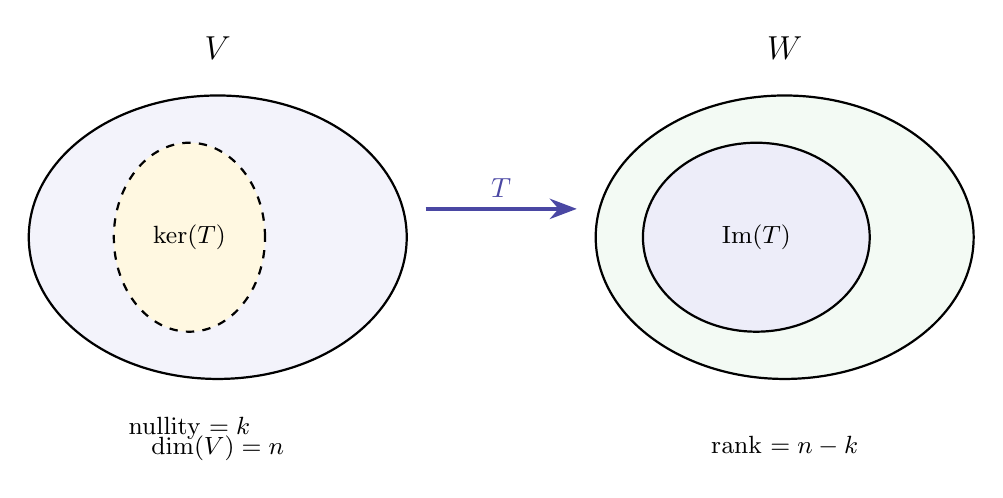
\begin{tikzpicture}[>=Stealth, scale=1.2]
  % V
  \draw[thick,fill=lightblue!50] (0,0) ellipse (2cm and 1.5cm);
  \node[font=\large\bfseries] at (0,2) {$V$};
  
  % ker T inside V
  \draw[thick,fill=prereqbg,dashed] (-0.3,0) ellipse (0.8cm and 1cm);
  \node[font=\small\bfseries] at (-0.3,0) {$\ker(T)$};
  
  % W
  \draw[thick,fill=examplebg!50] (6,0) ellipse (2cm and 1.5cm);
  \node[font=\large\bfseries] at (6,2) {$W$};
  
  % Im T inside W
  \draw[thick,fill=lightblue!80] (5.7,0) ellipse (1.2cm and 1cm);
  \node[font=\small\bfseries] at (5.7,0) {$\operatorname{Im}(T)$};
  
  % Arrow
  \draw[->,thick,accentblue,line width=1.5pt] (2.2,0.3) -- (3.8,0.3) 
    node[midway,above,font=\bfseries] {$T$};
  
  % Labels
  \node[font=\small,below] at (0,-2) {$\dim(V) = n$};
  \node[font=\small,below] at (-0.3,-1.8) {nullity $= k$};
  \node[font=\small,below] at (6,-2) {rank $= n - k$};
\end{tikzpicture}
\end{center}

\end{document}
